\chapter{Estado da Arte}

Neste capítulo é apresentado o estado da arte relativo ao contexto desta dissertação. 

\section{Introdução ao problema}

A plataforma \gls{clav} pode ser divididas em 3 eixos principais:

\begin{enumerate}
    \item \textbf{Frontend}
    Responsável pela interação dos utilizadores com plataforma, bem como chamadas à \gls{api}, podendo esta ser de cariz público ou privado, através do acesso a certas funcionalidades da plataforma (por exemplo: listagens de utilizadores, entidades, legislações, etc).
    
    \item \textbf{Backend}
    Desenvolvido em \emph{NodeJS}, este é responsável por satisfazer os serviços requisitados pelo \emph{Frontend}. Inclui toda a lógica da aplicação, como a camada de acesso a dados, leitura e armazenamento de informação.
    
    \item \textbf{API de dados}
    Responsável pela comunicação e gestão de pedidos dos utilizadores da plataforma, sendo que a sua principal função é servir de elo de ligação entre os resultados guardados em base de dados e o \emph{Frontend} disponibilizado aos utilizadores.
\end{enumerate}

Devido à natureza dos dados presentes na plataforma \gls{clav}, foi necessário proceder a uma correta e estruturada implementação de diversos mecanismos de segurança e proteção contra uso indevido de dados.

\cleardoublepage
%\section{Soluções adoptadas}
%De modo a oferecer um nível de segurança adequado à plataforma, foram adotadas várias medidas de segurança, sendo estas explicadas em mais detalhe nas subsecções seguintes.

\section{Gestão de utilizadores}

A gestão de utilizadores é feita através da combinação entre o middleware\footnote{Middleware é um software que funciona como intermediário entre dois programas.} designado por \emph{Passport} e a base de dados não-relacional\footnote{Estilo de base de dados livres de esquema, capazes de maior escalabilidade que as base de dados tradiconais.} implementada em \emph{MongoDB}.

Devido à informação sensível que pode ser guardada na mesma, campos como a password são, naturalmente, encriptados recorrendo a técnicas discutidas posteriormente.

%\subsubsection{Passport}
O \emph{Passport} é um middleware de autenticação, desenvolvido para \emph{NodeJS}, com mais de 500 estratégias\footnote{Uma estratégia pode ser interpretado como um mecanismo único de autenticação.} diferentes de autenticação. Foi criado para solucionar um único problema: \textbf{autenticar pedidos}.

Devido à natureza do \emph{Passport}, este é extremamente fácil de implementar numa dada aplicação, devido ao seu forte encapsulamento e ao facto de delegar qualquer funcionalidade, que não seja a autenticação, para a aplicação.

Devido à natureza das aplicações Web modernas, a autenticação pode ser feita por diversas estratégias. A estratégia utilizada neste projeto recaiu sobre a escolha mais "tradicional", uma autenticação local com campos para \emph{username} e \emph{password}.

Embora com o aumento exponencial da popularidade de implementações de autenticação baseadas em redes sociais, através de protocolos baseados em \emph{OAuth}\footnote{Protocolo open-source que permite autenticação de forma standard e segura, entre aplicações desktop, web e mobile.}, tais como \emph{Google+} e \emph{Facebook}, foi decidido desde uma fase inicial que tais estratégias não seriam consideradas devido ao carácter profissional da plataforma.

Devido a cada aplicação possuir necessidades diferentes, o \emph{Passport} guarda cada estratégia de autenticação em módulos independentes, deixando assim a cargo do programador que estratégias empregar, sem criar dependências desnecessárias.

De seguida será apresentada a forma como as passwords dos utilizadores estão a ser protegidas.

\cleardoublepage
\subsection{Introdução à encriptação}

Em qualquer aplicação no mundo real, é impensável guardar dados sensíveis, como passwords, em formato \emph{plain-text}. Daí surgiu a necessidade de proteger informação sensível através de métodos designados por \emph{hashing}\footnote{Uma função hash é um algoritmo que mapeia dados de comprimento variável para dados de comprimento fixo.}.\\

\begin{figure}[h]
    \centering
    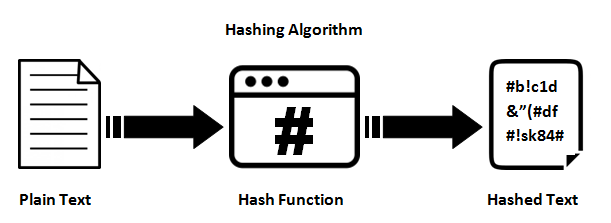
\includegraphics[width=0.75\textwidth]{img/bcrypt/Hashing.png}
    \caption{Representação de uma função de \emph{hash}. ADICIONAR FONTE}
\end{figure}

Em geral, o \emph{hashing} é caraterizado como uma operação de sentido único, através da qual se gera um resultado único, impossível de reverter para o texto original.
Embora esta noção esteja correta e seja de facto impossível, através de um texto já processado por uma função de \emph{hash}, reconstruir o texto original em questão, este não é infalível.

\cleardoublepage
\subsubsection{Vulnerabilidades}

Para exemplificar vulnerabilidades existentes nas funções criptográficas que recorrem apenas ao \emph{hashing} de passwords, vamos recorrer ao algoritmo \textbf{SHA-1}, pertencente à familia de algoritmos \gls{sha}.

O principal problema das funções da família \gls{sha} assenta no facto de que foram desenvolvidas para serem computacionalmente rápidas. A rapidez com que uma função pode calcular \emph{hashes}, tem um impacto imediato e significativo na quão seguro uma password é.

Embora cálculos mais rápidos levem ao desenvolvimento de algoritmos mais eficientes a nível de computação, também abrem portas a ataques \emph{bruteforce}. Atualmente, com o auxilio de \gls{cpu} e \gls{gpu} modernas, é possível calcular milhões, ou até bilhões de \emph{hashes} por segundo.

Outro problema assenta no facto que qualquer função responsável por \emph{hashing}, para o mesmo texto, retorna sempre o mesmo resultado de \emph{hash}, como podemos verificar na tabela seguinte.

\begin{center}
    \begin{tabular}{ |p{2cm}|p{2cm}|p{8cm}|  }
        \hline
        \multicolumn{3}{|c|}{Resultados do algoritmo SHA-1} \\
        \hline
        Utilizador & Password & \emph{Hashed} password\\
        \hline
        \textcolor{red}{António} & \textcolor{red}{12345} & \textcolor{red}{\textbf{8cb2237d0679ca88db6464eac60da96345513964}}\\
        Alice & sup3rs3gur4 & 0ce594a80be23686fa95527e219ff162291f80f0\\
        Manuel & uncrackabl3 & c4f9036ecefde84b5a8dc4296abbab1a6c53be60\\
        \textcolor{red}{Gustavo} & \textcolor{red}{12345} & \textcolor{red}{\textbf{8cb2237d0679ca88db6464eac60da96345513964}}\\
        Joana & 1a2b3c4d & b01afc2b077956acc69f99e0b7df1cb70cb01331\\
        \hline
    \end{tabular}
\captionof{table}{Aplicação do algoritmo \emph{SHA-1} a um conjunto de passwords.}\label{tab:sha1} 
\end{center}

Como exemplificado na Tabela \ref{tab:sha1}, o utilizador \textbf{António} e \textbf{Gustavo} partilham a mesma password, logo o resultado após o \emph{hashing} da mesma é idêntico. 

Embora passwords idênticas sejam extremamente comuns, o facto do \emph{hash} resultante ser idêntico apresenta um fator de risco muito mais elevado do que as passwords serem idênticas, pois estaria a expor um número exorbitante de utilizadores a uma grave falha de segurança.

Porém, o simples acto de \emph{hashing} de passwords não é uma solução segura. Este rapidamente foi descartado devido a ser extremamente suscetível a ataques baseado em \emph{rainbow tables}, também conhecidos por \emph{ataques de dicionário}.

Este ataque tem como base o facto de algoritmos como o \emph{SHA-1} ser extremamente rápido e eficiente, sendo que em vez de calcular em tempo real \emph{hashes} aleatórios, utilizam valores de hash pré-calculados para toda e qualquer possível combinação de caracteres, utilizando para validação o método \emph{bruteforce}.

Esta vulnerabilidade foi de tão larga escala, que poderia quebrar \emph{99.9\%} de todas as combinações possíveis de 14 caracteres alfanuméricos em 11 minutos (utilizando a \emph{rainbow table} menos extensa, sendo que com tabelas mais extensas esta figura descia consideravelmente).


%\cleardoublepage
\subsubsection{Melhorias no processo de hashing}

De modo a solucionar o problema anterior, é necessário implementar uma função de \emph{hashing} mais lenta, que seja eficaz na proteção de informação e capaz de abrandar, ou evitar possíveis ataques. Também é necessário que esta função seja adaptativa, ou seja, que devido a avanços tecnológicos em hardware esta se possa adaptar para ter um desempenho similar aos níveis atuais.

De modo a solucionar o problema proveniente de ataques \emph{bruteforce} baseados no uso de \emph{rainbow tables}, foi necessário diversificar ainda mais os \emph{hashes} gerados. Para tal foi adicionado um \emph{salt}, de modo a fazer qualquer password verdadeiramente única.

De acordo com a \gls{owasp}, o \emph{salt} é um valor aleatório de tamanho fixo, considerado criptograficamente forte, que é adicionado ao input de uma dada função de \emph{hash}, independentemente deste do input ser ou não único.

Na tabela seguinte podemos verificar a importância de utilizar a técnica de \emph{salting} juntamente com o \emph{hashing} de passwords.

\begin{center}
    \begin{tabular}{ |p{1.7cm}|p{2cm}|p{1.5cm}|p{8cm}|  }
        \hline
        \multicolumn{4}{|c|}{Resultados do algoritmo SHA-1 c/ salting} \\
        \hline
        Utilizador & Password & Salt &\emph{Hashed} password + \textbf{salt}\\
        \hline 
        \textcolor{red}{António} & \textcolor{red}{12345} & r8ZGQH & c783b62c876b77310818b3b4cc6863ca008f7d10\\
        Alice & sup3rs3gur4 & yvL9H8 & d68c7166f916b91b66dda685e8eee1af70528933\\
        Manuel & uncrackabl3 & C4uHRv & 87d8e4e7ae79ab2487133a6513e35cb511687d5a\\
        \textcolor{red}{Gustavo} & \textcolor{red}{12345} & jKM2Lh & f69e3288fc17c383cab12aa78a725d675610e81a\\
        Joana & 1a2b3c4d & WNj7Vt & 866038b3d43de9a9b0b49a6ee1ffc6cbf64d3c6d\\
        \hline
    \end{tabular}
\captionof{table}{Aplicação do algoritmo \emph{SHA-1} com auxílio de \emph{salting} a um conjunto de passwords.}\label{tab:sha1_salt} 
\end{center}

Como exemplificado na Tabela \ref{tab:sha1_salt}, embora o utilizador \textbf{António} e \textbf{Gustavo} partilhem a mesma password, o resultado do \emph{hashing} é diferente.

Facilmente chegamos à conclusão que o \emph{salting} é essencial para manter a segurança de informação importante como passwords, pois um conjunto infinito de passwords idênticas nunca terão o mesmo \emph{hash}.

Embora seja teoricamente possível quebrar este tipo de combinação, esta requer poder computacional exponencialmente maior que um simples ataque \emph{rainbow table}, visto que o \emph{salt} é totalmente aleatório, tornando qualquer ataque inviável.

Em suma, o método de autenticação ideal deve implementar ambos estes métodos, \emph{hashing} e \emph{salting}, sendo que um dos métodos mais comuns e seguros da atualidade, é o \emph{bcrypt}, tornando-a no perfeito candidato para utilização neste projeto.

\cleardoublepage
\subsection{bcrypt}

De modo a solucionar os problemas referidos na secção anterior, foi necessário proceder ao desenvolvimento de uma função criptográfica que não só solucionasse o problema relacionado com ataques via \emph{rainbow tables}, mas também fosse capaz de acompanhar os avanços tecnológicos a nível computacional.

Para tal, Niels Provos e David Mazières desenvolveram a função de \emph{hashing} designada por \textbf{bcrypt}. Esta foi apresentada em 1999 na \gls{usenix}, sendo uma função baseada na cifra \emph{Blowfish}, desenvolvia por Bruce Schneier e apresentada em 1993.

Além de incorporar um \emph{salt} para proteger contra ataques via \emph{rainbow tables}, esta foi desenvolvida para ser uma função adaptável, sendo que o número de iterações pode ser incrementado de modo a aumentar o número de ciclos máquina necessários para o cálculo do \emph{hash}. 

\begin{algorithm}
    \caption{Pseudo código do algoritmo \emph{bcrypt}.}
    \begin{algorithmic}[1]
        \Function{bcrypt}{cost, salt, pwd}
        \State $state\gets EksBlowfishSetup(cost,salt,key)$
        \State $ctext\gets OrpheanBeholderScryDoubt$
        \State \textbf{repeat}(64)
        \State \indent $ctext\gets EncryptECB(state, ctex)$
        \State \textbf{return} Concatenate(cost, salt, ctext)
    \EndFunction
    \end{algorithmic}
\end{algorithm}

A combinação destas duas técnicas faz com que, até à data de publicação desta pré-dissertação, o algoritmo \emph{bcrypt} ainda não tenha sido quebrado, sendo que se trata do algoritmo escolhido por sistemas operativos como o \emph{OpenBSD} e \emph{SUSE Linux} para o \emph{hashing} das suas passwords.

Esta fama levou a que o \emph{bcrypt} seja considerado por muitos, o standard da indústria em termos de encriptação de passwords.

\cleardoublepage
\subsubsection{Funcionamento do bcrypt}

De modo a proporcionar uma forma de aumentar o tempo computacional o algoritmo \emph{bcrypt}, Niels Provos e David Mazières basearam-se na cifra \emph{Blowfish} já existente, criando assim uma versão designada por \emph{Eksblowfish} (\textit{\textbf{Expensive key schedule} Blowfish}).

\begin{algorithm}
    \caption{Pseudo código do algoritmo \emph{EksBlowfish}.}
    \begin{algorithmic}[1]
        \Function{EksBlowfishSetup}{cost, salt, key}
        \State $state\gets InitState()$
        \State $state\gets ExpandKey(state, salt, key)$
        \State \textbf{repeat}($2^{cost}$)
        \State \indent $state\gets ExpandKey(state, 0, salt)$
        \State \indent $state\gets ExpandKey(state, 0, key)$
        \State \textbf{return} state
    \EndFunction
    \end{algorithmic}
\end{algorithm}

Esta alteração à cifra \emph{Blowfish} não foi feita com o intuito de a tornar criptograficamente mais forte, mas sim alterar a forma como a \emph{key} é calculada.

Tendo em consideração que a \emph{key} é um valor aleatório variável entre 1 e 72 bytes, inclusive, esta alteração torna o cálculo da \emph{key} demoroso a nível computacional (\textbf{Expensive}).

De modo a prolongar o tempo de execução desta função, é aplicada a expansão da \emph{key} $2^{cost}$ vezes. Esta alteração é a maior distinção entre o algoritmo \emph{Blowfish} original e o \emph{Eksblowfish}, sendo a causa do \emph{bcrypt} ser considerado um algoritmo adaptável.

No gráfico seguinte, podemos ver uma relação entre o facto de custo e o tempo de execução do algoritmo \emph{bcrypt}.

\begin{center}
    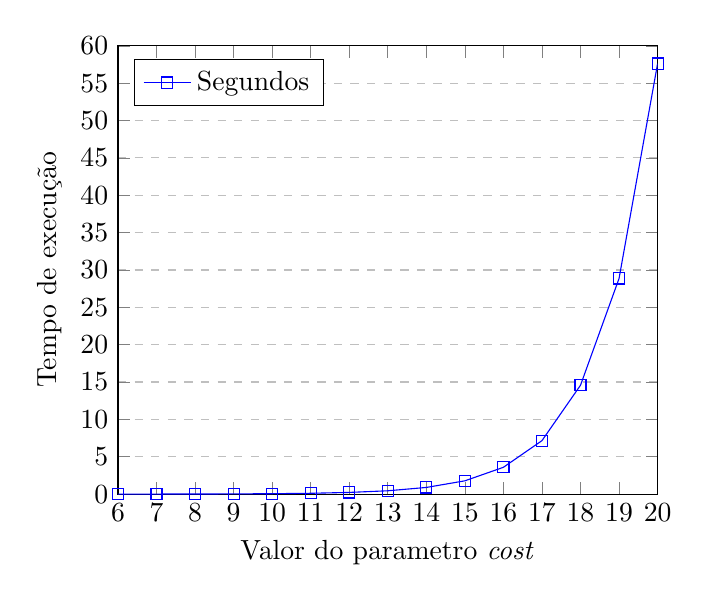
\begin{tikzpicture}
        \begin{axis}[
            xlabel={Valor do parametro \emph{cost}},
            ylabel={Tempo de execução},
            xmin=6, xmax=20,
            ymin=0, ymax=60,
            xtick={6,7,8,9,10,11,12,13,14,15,16,17,18,19,20},
            ytick={0,5,10,15,20,25,30,35,40,45,50,55,60},
            legend pos=north west,
            ymajorgrids=true,
            grid style=dashed,
        ]
        \addplot[
            color=blue,
            mark=square,
            ]
            coordinates {
            (6,0.003622)(7,0.007590)(8,0.013918)(9,0.028723)(10,0.055023)(11,0.110837)(12,0.226982)(13,0.446507)(14,0.892617)(15,1.778647)(16,3.588397)(17,7.155973)(18,14.572114)(19,28.860461)(20,57.623139)
            };
            \legend{Segundos}
        \end{axis}
    \end{tikzpicture}
\end{center}

\cleardoublepage
\section{Autenticação através do Auth.Gov}

\subsection{SSL}
\subsection{TLS}


\section{Autenticação de pedidos via API}
\subsection{JSON Web Token}


\section{Autenticação backend}